\documentclass[a4paper,11pt]{article}

\usepackage[dutch]{babel}
\usepackage[utf8]{inputenc}
\usepackage{a4wide,graphicx}
\usepackage{eurosym}
\usepackage{listings}
\usepackage{color}
\usepackage{hyperref}
\usepackage{comment}
\usepackage{float}
\usepackage{framed}
\usepackage{graphicx}

\lstset{numbers=left}

\begin{document}

\title{Inkapseling van veelgebruikte datastructuren}
\date{}

\maketitle

\section{Stack}

\subsection{Uitleg}

De stack of stapel is een veelgebruikte datastructuur in computerprogramma's die met techniek te maken hebben.
Kenmerk van een stapel, bijvoorbeeld een stapel papier op je bureau, is dat wat je er als laatste oplegt, er ook makkelijk weer als eerste af te pakken is.
Een stack wordt ook wel \emph{lifo} genoemd: last in, first out.
Soms is dat niet handig, zoals bij rekeningen...

\begin{itemize}
\item Een geval waarin een stapel wel handig is, is als je wilt onthouden waar je mee bezig bent.
Je bent bijvoorbeeld een computerspel aan 't schrijven en hebt allerlei ideeen bedacht.
Die schrijf je op een briefje dat je op je bureau legt.

\item Halverwege blijkt dat je compilerversie te oud is om nog een nieuwe versie van een library te compileren.
Je schrijft op een ander briefje welke versie je moet installeren en legt dat er bovenop.

\item Als je met de installatie van de nieuwe compiler wilt beginnen,
blijkt dat hiervoor een nieuwere versie van je besturingssysteem nodig is.
Je schrijft op welke versie, en legt dat briefje bovenop de stapel.

\item Vervolgens download je een diskimage, maar daarna blijkt je harde schijf overvol.
Je zoekt op internet op welke je moet hebben en schrijft 't op.

\item Daarna ga na naar de website van HotRed en besteld de harde schijf.
Het bovenste briefje kan nu weg en het briefje met gegevens van het nieuwe besturingssysteem ligt bovenop.

\item Je download de juiste versie en gooit ook dat briefje weg.
Het briefje met de gegevens van de gewenste compiler ligt nu bovenop.

\item Je download de compiler en gooit ook dat briefje weg.
Voor je ligt het briefje met je ideeen voor het computergame.
Tijd voor koffie...
\end{itemize}

De situatie waarin taken worden opgeschort om eerst andere taken te doen komt veel voor in computerprogamma's.
Als een functie f een andere functie g aanroept, heb je precies die situatie.
Functie g kan weer functie h aanroepen en zo verder.
Als een bepaalde functie klaar is gaat de executie verder met de functie die deze functie aanriep.

De lokale variabelen, waaronder de parameters, die in een bepaalde functie nodig zijn worden voor elke call op de stack opgeslagen.
Zo'n verzameling lokale variabelen heet een stackframe.
Na het verlaten van de functie wordt het betreffende stackframe weer vrijgegeven.

Omdat elke aanroep z'n eigen stackframe creeert, is het mogelijk dat een functie zichzelf aanroept.
Dit heet recursie en kan, mits op de goede plaats toegepast, erg handig zijn.
Als een functie zichzelf te vaak aanroept raakt de stack vol: stack overflow.

\subsection{Oefening}

Een andere toepassing van een stack is het doen van berekeningen zonder gebruik van haakjes.
Er zijn rekenmachines die zo werken.
In plaats van
\begin{verbatim}
6 * (4 + 3) + 1 =
\end{verbatim}
type je dan
\begin{verbatim}
6 4 3 + * 1 +
\end{verbatim}
Dit is te realiseren met behulp van een stack.
Probeer op papier of met briefjes uit hoe dit zou kunnen werken.
Maak een Stack class, en instantieer deze om een rekenmachine te maken.
Maak in deze klasse gebruik van een Java array.
Test je rekenmachine grondig.
Een paar gebruikelijke termen: Iets op een stapel leggen heet \emph{push}.
Iets ervanaf halen heet \emph{pop}.
Je mag dingen vragen aan de docent en overleggen met anderen.
Maar zorg wel dat je weet hoe je eigen code werkt!

\section{Queue}

\subsection{Uitleg}

Een andere veel voorkomende datastructuur is de wachtrij of queue.
Bij een queue komt wat je er als eerste instopt, er ook als eerste weer uit.
Daarom wordt een queue ook wel \emph{fifo} genoemd: first in, first out.
Een queue is beter geschikt voor rekeningen dan een stack, als je tenminste van plan bent ze te betalen...

Queues komen veel voor in computerprogramma's, bijvoorbeeld als doorgeefluik tussen twee parallele processen.
Parallel wil in dit geval zeggen dat de computer ogenschijnlijk twee dingen tegelijk doet.
Omdat deze twee dingen niet altijd in de pas lopen, wisselen ze gegevens uit via wachtrijen:
gaat u maar in de rij staan bij het volgende loket, want mijn collega is even koffiedrinken.

De printer queue is een ander voorbeeld van een wachtrij.
Queue's kunnen vol raken of leeg zijn.
Als je iets uit een queue wilt halen, zul je moeten achterhalen of het er al in staat.
Daarom hebben queue objecten meestal een method om hierachter te komen, bijvoorbeeld \emph{size} of \emph{empty}.

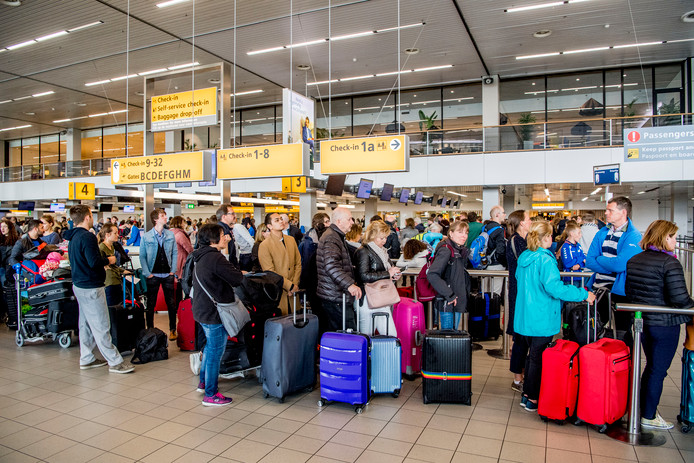
\includegraphics[width=15cm]{checkin}

\begin{framed}
Een rij mensen bij de incheckbalie van een luchthaven schuift meestal langzaam op richting knappe juffrouw met blauw pakje.
Ook alle koffers worden dan zuchtend weer een plaatsje naarvoren geschoven.
Bij gegevens in het hoofdgeheugen van een computer dient dit te worden voorkomen.
Alles vier bytes opschuiven bij een queue van twee gigabytes is een onnodig dure operatie.
Beter is 't de queue op z'n plek te laten en te onthouden waar de het eerste en 't laatste dataelement zich bevinden.
De dame van de incheckbalie loopt in dit geval langs de rij met een verrijdbare weegschaal voor de koffers en een labelprinter.
Wie is afgehandeld gaat uit de rij met z'n gewogen en gelabelde koffer en zet 'm ergens op een lopende band.
Op die plek waar mensen uit de rij gaan, komen er nieuwe mensen bij.
Niemand hoeft op te schuiven en iedereen kan rustig zittend op z'n koffer genieten van het uitzicht op alle rennende zakenlui.
Geen luchthaven is nog op dit idee gekomen, maar bij software queues is dit al lang gebruikelijk.
\end{framed}

\subsection{Oefening}

Maak een Queue class die de data niet opschuift, maar onthoudt waar er data bijkomt en waar deze aan de beurt is om uit de rij gehaald te worden.
Iets in de rij plaatsen gebeurt met \emph{put}, iets eruit halen gebeurt met \emph{get}.
Om deze opdracht te kunnen maken, kun je, naast een array, het beste de Java \emph{modulus} operator gebruiken.
Zoek op internet op hoe deze precies werkt.

Maak met behulp van je Queue class een Obfuscator class, die woorden op volgorde van aankomst omzet naar een onleesbare, maar decodeerbare string.
Maak een hoofdprogramma dat een zin op deze manier codeert en de gecodeerde woorden afdrukt.
Het moet mogelijk zijn woorden in ``kluitjes'' in te voeren en ze er in andere ``kluitjes'' uit te halen.
Met andere woorden: je obfuscator moet op woordniveau kunnen bufferen:
net als bij printopdrachten komen de woorden in een queue te staan waar ze zo af en toe (eventueel in kluitjes) worden uitgehaald.
Ook hier mag je weer dingen vragen en hulp zoeken.
Maar ook hier wordt weer van je verwacht dat je uiteindelijk regel voor regel kunt uitleggen hoe je code werkt.

\end{document}
